\documentclass[journal,12pt,onecolumn]{IEEEtran}
\usepackage{cite}
\usepackage{amsmath,amssymb,amsfonts,amsthm}
\usepackage{algorithmic}
\usepackage{graphicx}
\graphicspath{{./figs/}}
\usepackage{textcomp}
\usepackage{xcolor}
\usepackage{txfonts}
\usepackage{listings}
\usepackage{enumitem}
\usepackage{mathtools}
\usepackage{gensymb}
\usepackage{comment}
\usepackage{caption}
\usepackage[breaklinks=true]{hyperref}
\usepackage{tkz-euclide} 
\usepackage{listings}
\usepackage{gvv}                                        
%\def\inputGnumericTable{}                                 
\usepackage[latin1]{inputenc}     
\usepackage{xparse}
\usepackage{color}                                            
\usepackage{array}                                            
\usepackage{longtable}                                       
\usepackage{calc}                                             
\usepackage{multirow}
\usepackage{multicol}
\usepackage{hhline}                                           
\usepackage{ifthen}                                           
\usepackage{lscape}
\usepackage{tabularx}
\usepackage{array}
\usepackage{float}
\usepackage{booktabs}
\newtheorem{theorem}{Theorem}[section]
\newtheorem{problem}{Problem}
\newtheorem{proposition}{Proposition}[section]
\newtheorem{lemma}{Lemma}[section]
\newtheorem{corollary}[theorem]{Corollary}
\newtheorem{example}{Example}[section]
\newtheorem{definition}[problem]{Definition}
\newcommand{\BEQA}{\begin{eqnarray}}
\newcommand{\EEQA}{\end{eqnarray}}
\newcommand{\define}{\stackrel{\triangle}{=}}
\theoremstyle{remark}
\newtheorem{rem}{Remark}

\begin{document}
\title{
ASSIGNMENT 5: GATE 2025 \\
AG : Agricultural Engineering}
\author{EE25BTECH11047 - Ravula Shashank Reddy}
\maketitle
\renewcommand{\thefigure}{\theenumi}
\renewcommand{\thetable}{\theenumi}

\begin{enumerate}

\item Ravi had \underline{\hspace{2cm}} younger brother who taught at  \underline{\hspace{2cm}} university. 
He was widely regarded as \underline{\hspace{2cm}} honorable man.  
Select the option with the correct sequence of articles to fill in the blanks.

\hfill(GATE EE 2025)

\begin{multicols}{4}
\begin{enumerate}
\item a; a; an
\item the; an; a
\item a; an; a
\item an; an; a
\end{enumerate}
\end{multicols}

\item The CEO's decision to downsize the workforce was considered myopic 
because it sacrificed long-term stability to accommodate short-term gains.  
Select the most appropriate option that can replace the word "myopic"
without changing the meaning of the sentence.  

\hfill(GATE EE 2025)

\begin{multicols}{4}
\begin{enumerate}
\item visionary
\item shortsighted
\item progressive
\item innovative
\end{enumerate}
\end{multicols}

\item The average marks obtained by a class in an examination were calculated as 30.8. 
However, while checking the marks entered, the teacher found that the marks of one 
student were entered incorrectly as 24 instead of 42. After correcting the marks, 
the average becomes 31.4. How many students does the class have?

\hfill(GATE EE 2025)

\begin{multicols}{4}
\begin{enumerate}
\item 25
\item 28
\item 30
\item 32
\end{enumerate}
\end{multicols}

\item Consider the relationships among P, Q, R, S, and T:\\  
 P is the brother of Q.\\  
 S is the daughter of Q.\\  
 T is the sister of S. \\
 R is the mother of Q. \\ 
The following statements are made based on the relationships given above.\\  
(1) R is the grandmother of S.  \\
(2) P is the uncle of S and T.  \\
(3) R has only one son.  \\
(4) Q has only one daughter.\\  
Which one of the following options is correct?

\hfill(GATE EE 2025)

\begin{multicols}{2}
\begin{enumerate}
\item Both (1) and (2) are true.
\item Both (1) and (3) are true.
\item Only (3) is true.
\item Only (4) is true.
\end{enumerate}
\end{multicols}
\newpage
\item According to the map shown in the figure, which one of the following statements is correct?  \\
\begin{figure}
    \centering
    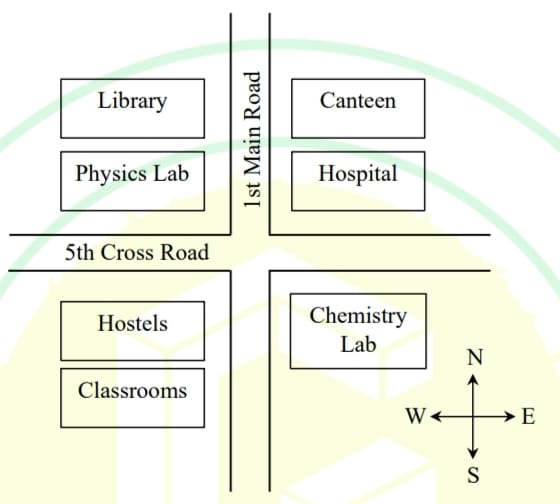
\includegraphics[width=0.3\linewidth]{figs/Fig 1.jpg}
    \caption{}
    \label{fig:placeholder}
\end{figure}

\hfill(GATE EE 2025)

\begin{enumerate}
\item The library is located to the northwest of the canteen.
\item The hospital is located to the east of the chemistry lab.
\item The chemistry lab is to the southeast of physics lab.
\item The classrooms and canteen are next to each other.
\end{enumerate}

\item "I put the brown paper in my pocket along with the chalks, and possibly other things. 
I suppose every one must have reflected how primeval and how poetical are the things that one carries in one's pocket: the pocket-knife, for instance the type of all human tools, the infant of the sword. Once I planned to write a book of poems entirely about the things in my pocket. But I found it would be too long: and the age of the great epics is past."  
(From G.K. Chesterton's "A Piece of Chalk")  

Based only on the information provided in the above passage, which one of the following statements is true?

\hfill(GATE EE 2025)

\begin{enumerate}
\item The author of the passage carries a mirror in his pocket to reflect upon things.
\item The author of the passage had decided to write a poem on epics.
\item The pocket-knife is described as the infant of the sword.
\item Epics are described as too inconvenient to write.
\end{enumerate}

\item In the diagram, the lines QR and ST are parallel to each other. 
The shortest distance between these two lines is half the shortest distance between the point P and line QR. 
What is the ratio of the area of the triangle PST to the area of the trapezium SQRT?

    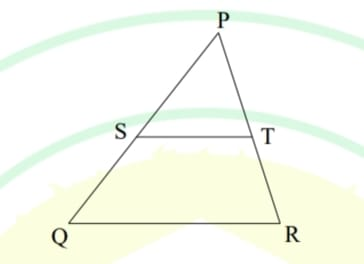
\includegraphics[width=0.3\linewidth]{figs/Fig 7.jpg}

\hfill(GATE EE 2025)

\begin{multicols}{4}
\begin{enumerate}
\item 1/3
\item 1/4
\item 2/5
\item 1/2
\end{enumerate}
\end{multicols}

\item A fair six-faced dice, with the faces labelled '1', '2', '3', '4', '5', and '6', is rolled thrice. 
What is the probability of rolling '6' exactly once?

\hfill(GATE EE 2025)

\begin{multicols}{4}
\begin{enumerate}
\item 75/216
\item 1/6
\item 1/18
\item 25/216
\end{enumerate}
\end{multicols}

\item A square paper, shown in figure (I), is folded along the dotted lines as shown in the figures (II) and (III). 
Then a few cuts are made as shown in figure (IV). 
Which one of the following patterns will be obtained when the paper is unfolded?  

 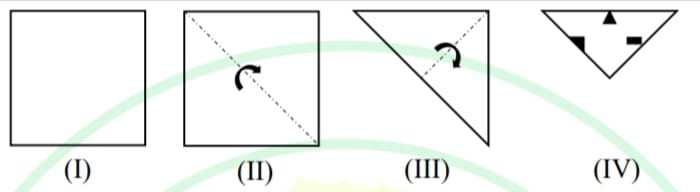
\includegraphics[width=0.5\linewidth]{figs/Fig 2.jpg}
 
\hfill(GATE EE 2025)

\begin{multicols}{2}
\begin{enumerate}

\item  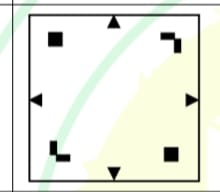
\includegraphics[width=0.3\linewidth]{figs/Fig 3.jpg}
\item  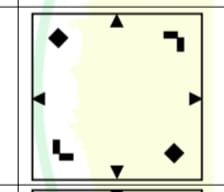
\includegraphics[width=0.3\linewidth]{figs/Fig 4.jpg}
\item  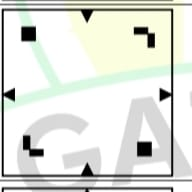
\includegraphics[width=0.3\linewidth]{figs/Fig 5.jpg}
\item  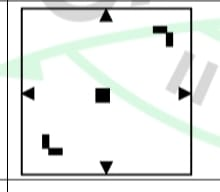
\includegraphics[width=0.3\linewidth]{figs/Fig 6.jpg}
\end{enumerate}
\end{multicols}

\item A shop has 4 distinct flavors of ice-cream. One can purchase any number of scoops of any flavour. 
The order in which the scoops are purchased is inconsequential. 
If one wants to purchase 3 scoops of ice-cream, in how many ways can one make that purchase?  

\hfill(GATE EE 2025)

\begin{multicols}{4}
\begin{enumerate}
\item 4
\item 20
\item 24
\item 48
\end{enumerate}
\end{multicols}


\item If a, b, and c are the roots of $2x^3 - 3x^2 + px - 1 = 0$ and sum of the two roots is 1, the value of $p$ is:

\hfill(GATE EE 2025)

\begin{multicols}{4}
\begin{enumerate}
\item 2
\item 1
\item 3
\item 1/3
\end{enumerate}
\end{multicols}

\item If the matrix \myvec {x & -3 \\ 2 & x-5 } is singular, sum of the values of $x$ is:

\hfill(GATE EE 2025)

\begin{multicols}{4}
\begin{enumerate}
\item 5
\item 6
\item 0
\item -1
\end{enumerate}
\end{multicols}

\item $\dfrac{s}{s^2+a^2}$ is the Laplace transform of:

\hfill(GATE EE 2025)

\begin{multicols}{4}
\begin{enumerate}
\item $\cos at$
\item $\sin at$
\item $\sinh at$
\item $\cosh at$
\end{enumerate}
\end{multicols}

\item \begin{align*}
    y'' + p(x)y' + q(x)y = r(x)
\end{align*} is a \underline{\hspace{2cm}}ordinary differential equation.

\hfill(GATE EE 2025)

\begin{multicols}{2}
\begin{enumerate}
\item second order, nonhomogeneous, and linear
\item second order, homogeneous, and linear
\item second order, homogeneous, and nonlinear
\item first order, nonhomogeneous, and linear
\end{enumerate}
\end{multicols}

\item The median of the following set of numbers: 154, 130, 144, 137, 156, 146, 138, 149, 160, 138 is:

\hfill(GATE EE 2025)

\begin{multicols}{4}
\begin{enumerate}
\item 145.0
\item 145.2
\item 151.0
\item 146.0
\end{enumerate}
\end{multicols}

\item Which of the following method is used for the geophysical exploration of groundwater:

\hfill(GATE EE 2025)

\begin{multicols}{2}
\begin{enumerate}
\item Electric Resistivity method
\item Test Boring method
\item Tracer method
\item Remediation method
\end{enumerate}
\end{multicols}

\item Identify the correct statement related to tape correction in chain surveying:

\hfill(GATE EE 2025)

\begin{multicols}{2}
\begin{enumerate}
\item Wrong alignment correction is always positive.
\item Sag correction is always negative.
\item Slope of tape correction is always positive.
\item Temperature correction is always negative.
\end{enumerate}
\end{multicols}

\item The sphericity of a cylindrical potato sample having diameter of 1.0 cm and length of 5.0 cm is closest to:

\hfill(GATE EE 2025)

\begin{multicols}{4}
\begin{enumerate}
\item 0.98
\item 0.70
\item 0.31
\item 0.17
\end{enumerate}
\end{multicols}

\item The condition of refrigerant at the exit of the compressor in a vapor compression refrigeration system is:

\hfill(GATE EE 2025)

\begin{multicols}{4}
\begin{enumerate}
\item Saturated liquid
\item Wet vapor
\item Dry saturated vapor
\item Superheated vapor
\end{enumerate}
\end{multicols}

\item While sowing mustard seeds (bulk density = 800 kgm$^{-3}$), a four-row fluted roller type seed drill with 25 cm row spacing operates at a speed of 2.5 kmh$^{-1}$. For a desired seed rate of 5.0 kgha$^{-1}$, the flowrate of seeds from the machine in m$^3$h$^{-1}$ is:

\hfill(GATE EE 2025)

\begin{multicols}{4}
\begin{enumerate}
\item $0.391 \times 10^{-3}$
\item $1.172 \times 10^{-3}$
\item $1.563 \times 10^{-3}$
\item $1.953 \times 10^{-3}$
\end{enumerate}
\end{multicols}


\item By tripling the RMS sound pressure, the resulting increase in the sound pressure level in dB is closest to:

\hfill(GATE EE 2025)

\begin{multicols}{4}
\begin{enumerate}
\item 9.54
\item 6.02
\item 4.77
\item 3.01
\end{enumerate}
\end{multicols}

\item While studying vertical motion imparted to the base of tractor seat, $\theta$ (radian) is considered as rotation about tractor's CG and $R$ is considered as longitudinal distance from operator's seat to the tractor's CG. For a small value of $\theta$, the term $R\theta$ represents the vertical motion resulting from tractor's \underline{\hspace{2cm}}.

\hfill(GATE EE 2025)

\begin{multicols}{4}
\begin{enumerate}
\item pitch motion
\item roll motion
\item yaw motion
\item lateral motion
\end{enumerate}
\end{multicols}

\item In rice milling, the rubber roll sheller is used for:

\hfill(GATE EE 2025)

\begin{multicols}{2}
\begin{enumerate}
\item Separating paddy from brown rice
\item Removal of bran adhering to rice kernels
\item Separating husk layer from paddy grains
\item Removal of husk layer from white rice
\end{enumerate}
\end{multicols}

\item In general, result(s) of blanching fresh fruits and vegetables is/are:

\hfill(GATE EE 2025)

\begin{enumerate}
\item Complete elimination of microorganisms
\item Removal of entrapped air pockets between plant tissues
\item Leaching of nutrients
\item Inactivation of enzymes
\end{enumerate}


\item Identify the adverse effect(s) due to soil salinity or alkalinity or both:

\hfill(GATE EE 2025)

\begin{multicols}{2}
\begin{enumerate}
\item Low yields of crops
\item Increased infiltration leading to waterlogging
\item Poor quality of fodder
\item Limited type of crops can be grown
\end{enumerate}
\end{multicols}

\item Match the terms in Column I with the suitable hydrometeorological variables in Column II.
\begin{center}
\begin{tabular}{|c|l|c|l|}
\hline
\textbf{Column 1} & & \textbf{Column 2} & \\ \hline
P & Isopleth & 1 & Rainfall \\ \hline
Q & Isobath & 2 & Pressure \\ \hline
R & Isohyet & 3 & Evapotranspiration \\ \hline
S & Isochrone & 4 & Groundwater \\ \hline
T & Isobar & 5 & Surface runoff \\ \hline
\end{tabular}
\end{center}

\hfill(GATE EE 2025)

\begin{multicols}{2}
\begin{enumerate}
\item P-4, Q-3, R-1, S-5, T-2
\item P-5, Q-4, R-1, S-3, T-2
\item P-3, Q-4, R-1, S-5, T-2
\item P-3, Q-4, R-2, S-5, T-1
\end{enumerate}
\end{multicols}

\item Identify correct statement(s) for sprinkler irrigation:

\hfill(GATE EE 2025)

\begin{multicols}{2}
\begin{enumerate}
\item Excessive topsoil erosion is involved.
\item Fertilizer can be applied with water.
\item No excess cost of land preparation is involved.
\item Evapotranspiration loss is minimum.
\end{enumerate}
\end{multicols}

\item Which of the following method(s) is/are generally used in spark ignition engines for evaluating volatility?

\hfill(GATE EE 2025)

\begin{multicols}{2}
\begin{enumerate}
\item Distillation test
\item Motor method
\item Pensky Martens closed tester
\item Reid vapor pressure test
\end{enumerate}
\end{multicols}

\item The nominal radius of the rear wheels of a 2WD tractor is 0.5 m. The rolling radius of the tire is 6\% less than the nominal radius. While conducting a field test, if the actual distance covered for 20 revolutions of the rear wheel is found to be 56 m, the rear wheel slip is \underline{\hspace{2cm}}.\\(Rounded off to 2 decimal places).

\hfill(GATE EE 2025)

\item Front wheel pivot points of a 2WD tractor are 1.2 m apart. When making turn on a flat concrete surface, the inner front wheel makes 50$^\circ$ and the outer front wheel makes 35$^\circ$ steering angles. To ensure turning without front wheel skid, the wheel base of the tractor should be \underline{\hspace{2cm}}m. (Rounded off to 2 decimal places)

\hfill(GATE EE 2025)

\item An unconfined aquifer having a hydraulic conductivity of 12 m.day$^{-1}$ covers an area of 1.0 ha. When this aquifer is pumped, it releases 6000 m$^3$ of water and the water table drops from 3 m to 7 m below the ground level. The specific yield of the aquifer is\underline{\hspace{2cm}}. (Answer in integer)

\hfill(GATE EE 2025)

\item Apple slices are dried from a moisture content of 65\% (dry basis) to 10\% (dry basis) in a hybrid solar dryer under falling rate period. The apple slices have a drying rate constant of $1/104$ min$^{-1}$. Considering an equilibrium moisture content of 2\% (dry basis), the time required for drying is \underline{\hspace{2cm}} minutes. (Rounded off to 2 decimal places)

\hfill(GATE EE 2025)

\item The quantity of water needed to increase the moisture content of 50 kg paddy grains from 13\% (dry basis) to 35\% (dry basis) in the hydrothermal treatment process is\underline{\hspace{2cm}} kg. (Rounded off to 2 decimal places)

\hfill(GATE EE 2025)

\item Considering acceleration due to gravity as 9.81 m.s$^{-2}$ and $\pi$ as 3.14, the critical speed of a ball mill having 3600 mm mill diameter and 160 mm ball diameter is \underline{\hspace{2cm}} rpm. (Answer in integer)

\hfill(GATE EE 2025)

\item Three straight metal wires, AC, BC and CD, having same length, diameter and thermal conductivity are connected as shown in the figure. Heat flows from points 'A' and 'B' to point 'C' and from point 'C' to 'D'. Temperatures at points A, B and D are 100{\degree}C, 100{\degree}C and 40 {\degree}C, respectively. Assuming steady-state condition and no heat loss from the wires, the temperature at point 'C' is \underline{\hspace{2cm}} {\degree}C. (Answer in integer)

\hfill(GATE EE 2025)

 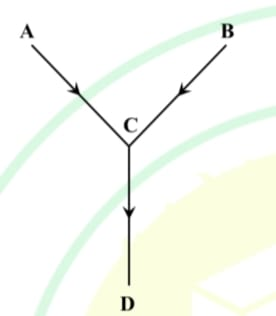
\includegraphics[width=0.3\linewidth]{figs/Fig 8.jpg}
\item The series has the sum : \begin{align*}
   \sum_{n=0}^{r} q^n = 1 + q + q^2 + \cdots 
\end{align*}

\hfill(GATE EE 2025)

\begin{multicols}{4}
\begin{enumerate}
\item $\dfrac{1}{1-q} - \dfrac{q^{r+1}}{1-q}$
\item $\dfrac{1}{q-1} + \dfrac{q^{r+1}}{q-1}$
\item $\dfrac{1}{1-q} + \dfrac{q^{r+1}}{1-q}$
\item $\dfrac{1}{q-1}$
\end{enumerate}
\end{multicols}

\item The value of $\lim_{x \to 0} \dfrac{x \cos x - \sin x}{x^2 \sin x}$ is:

\hfill(GATE EE 2025)

\begin{multicols}{4}
\begin{enumerate}
\item $-\dfrac{1}{3}$
\item $\dfrac{1}{3}$
\item 3
\item -3
\end{enumerate}
\end{multicols}

\item If $u = x^4 + y^4 + 3x^2y^2$, the value of $\left(x \dfrac{\partial u}{\partial x} + y \dfrac{\partial u}{\partial y}\right)^{-1}$ is:

\hfill(GATE EE 2025)

\begin{multicols}{4}
\begin{enumerate}
\item $4u$
\item 0
\item $\dfrac{1}{4u}$
\item $2u$
\end{enumerate}
\end{multicols}

\item Steady flow condition in a confined aquifer occurs when:

\hfill(GATE EE 2025)

\begin{enumerate}
\item the rate of recharge is more than the rate of groundwater discharge.
\item the rate of recharge is equal to the rate of groundwater discharge.
\item the rate of recharge is less than the rate of groundwater discharge.
\item the pumping rate is more than the safe yield of the aquifer.
\end{enumerate}


\item Lysimeter is an instrument used to measure the following process(es):

\hfill(GATE EE 2025)

\begin{multicols}{4}
\begin{enumerate}
\item Evaporation
\item Infiltration
\item Evapotranspiration
\item Deep percolation
\end{enumerate}
\end{multicols}


\item The assumption(s) which is/are not correct for deriving the Plank's equation for estimation of food freezing time:

\hfill(GATE EE 2025)

\begin{enumerate}
\item Ice front moves from the freezing medium into the food block at a uniform rate.
\item Physical property data of food material are accurate.
\item Initially the whole food material is at a distinct freezing point.
\item Sensible heat changes during the freezing process are sufficiently high.
\end{enumerate}

\item Match the following psychrometric processes (Column I) with the respective changes in thermodynamic properties (Column II) of air-water vapor mixture:

\begin{center}
\begin{tabular}{|l|l|l|l|}
\hline
\textbf{Column 1} & & \textbf{Column 2} & \\ \hline
1 & Sensible cooling & P & Dry bulb temperature increases and 
dew point temperature decreases \\ \hline
2 & Cooling and dehumidification & Q & Dry bulb temperature increases and dew point temperature increases \\ \hline
3 & Chemical dehumidification & R & Dry bulb temperature decreases and dew point temperature remains constant \\ \hline
4 & Heating and humidification & S & Dry bulb temperature decreases and dew point temperature decreases\\ \hline

\end{tabular}
\end{center}

\hfill(GATE EE 2025)

\begin{multicols}{2}
\begin{enumerate}
\item 1-R, 2-S, 3-Q, 4-P
\item 1-P, 2-R, 3-S, 4-Q
\item 1-R, 2-S, 3-P, 4-Q
\item 1-P, 2-Q, 3-S, 4-R
\end{enumerate}
\end{multicols}

\item The value of $y$ at $x = 0.3$ and $y(x=0) = 0$ for the differential equation is \underline{\hspace{2cm}}. \begin{align*}
   \dfrac{dy}{dx} = 3y + 2e^x 
\end{align*}

\hfill(GATE EE 2025)

\item A flat plate solar collector located at Bhopal (23$^\circ$15'N, 77$^\circ$42'E) is tilted at an angle of 30$^\circ$ with the horizontal and facing due South. Considering hour angle as 45$^\circ$, the angle made by the beam radiation with normal to the collector plate on June 30, 2023 at 3:00 PM (Local Apparent Time) is \underline{\hspace{2cm}} degree. (Rounded off to 2 decimal places)

\hfill(GATE EE 2025)

\item A six-stage centrifugal pump delivers water at the rate of 150 L.s$^{-1}$ against a net pressure rise of 5003 kN.m$^{-2}$. The pump impeller rotates at 1450 rpm. If the acceleration due to gravity is 9.81 m.s$^{-2}$, the specific speed of the pump is\underline{\hspace{2cm}}. (Answer in integer)

\hfill(GATE EE 2025)

\item Water flows through a 90$^\circ$ V-notch weir having a discharge coefficient of 0.6. If the depth of water above the notch is 49 cm and the acceleration due to gravity is 9.81 m.s$^{-2}$, the discharge over the notch is \underline{\hspace{2cm}} m$^3$.s$^{-1}$. (Rounded off to 2 decimal places)

\hfill(GATE EE 2025)

\item The volume and voids ratio of an undisturbed soil sample are 100 cm$^3$ and 0.60, respectively. After oven drying, the mass of this sample is reduced from 185 g to 165 g without any shrinkage in the volume. If the specific gravity of this sample is 2.64, the degree of saturation of this soil is\underline{\hspace{2cm}}. (Rounded off to 2 decimal places)

\hfill(GATE EE 2025)

\item A 10 ha watershed experiences a rainfall of 15 mm, evapotranspiration of 5 mm, infiltration of 4.5 mm, deep percolation of 2.2 mm, detention storage of 0.5 mm, and other abstraction losses of 0.3 mm during the storm event. Neglecting other surface storages, the total overland flow generated from the watershed due to this storm event is \underline{\hspace{2cm}} m$^3$. (Answer in integer)

\hfill(GATE EE 2025)

\item To protect a wheat field from wind erosion, windbreaks of 2.7 m height are provided. The actual wind velocity at 15 m height perpendicular to the wind barrier is 9 m.s$^{-1}$ and the minimum wind velocity at 15 m height required to move the most erodible soil fraction is 9.6 m.s$^{-1}$. The distance of full protection from this windbreak is\underline{\hspace{2cm}} m. (Rounded off to 2 decimal places)

\hfill(GATE EE 2025)

\item A stable drop structure is designed with a base length of 5.7 m. The sum of vertical forces excluding uplift is 92.5 kN, sum of uplift forces is 72.5 kN, and sum of moments of all the horizontal and vertical forces about an axis passing through mid-section of base length is 60 kN.m. The eccentricity denoting the longitudinal distance between the centroid of base area and the point of application of resultant vertical load is\underline{\hspace{2cm}} m. (Rounded off to 2 decimal places)

\hfill(GATE EE 2025)

\item An 8 ha watershed receives rainfall intensities of 2.5, 3.6, 5.4, 3.3, 2.6 and 1.2 cm.h$^{-1}$ at successive intervals of 30 minutes. The corresponding surface runoff volume is estimated to be 4800 m$^3$. Neglecting initial abstraction losses, the W-index for this watershed is \underline{\hspace{2cm}} cm.h$^{-1}$. (Rounded off to 2 decimal places)

\hfill(GATE EE 2025)

\item A four-stroke diesel engine has a displacement volume of 6.0 L and it operates at 2300 rpm with 75\% mechanical efficiency. The indicated mean effective pressure is 800 kPa. If the engine has brake-specific fuel consumption of 320 g.h$^{-1}$.kW$^{-1}$, considering calorific value of the fuel as 44.6 MJ.kg$^{-1}$, the fuel equivalent power is \underline{\hspace{2cm}} kW. (Rounded off to 2 decimal places)

\hfill(GATE EE 2025)

\item An engine's torque-speed characteristics is given below:  
$T_{maxP} = 125$ N.m, $N_{maxP} = 2400$ rpm, $N_{HI} = 2600$ rpm  
$T_{max} = 160$ N.m, $N_{maxT} = 1450$ rpm  

The Governor's regulation is \underline{\hspace{2cm}}. (Rounded off to 2 decimal places)

\hfill(GATE EE 2025)

\item An engine, running at 1200 rpm, drives a 1.2 m diameter rigid wheel on a non-deformable surface at 5 km.h$^{-1}$ forward speed. The power is transmitted from engine to the wheel through a transmission gear box (gear ratio = 3:1), a differential (gear ratio = 4:1), and a final drive (gear ratio = n:1). Neglecting the deformation of the wheel and wheel slip, the value of $n$ is\underline{\hspace{2cm}}. (Rounded off to 2 decimal places)

\hfill(GATE EE 2025)

\item A solid round uniform diameter shaft is transmitting 25 kW power at 540 rpm. The maximum allowable shear stress of the shaft material is 35 MPa. If the maximum torque exceeds the mean torque by 20\%, neglecting the bending effect, the minimum shaft diameter is \underline{\hspace{2cm}} mm. (Rounded off to 2 decimal places)

\hfill(GATE EE 2025)

\item The height of CG of a 4WD tractor with equal tread (1.25 m) in front and rear is 0.85 m. The tractor overturns during turning at a speed of 18 km.h$^{-1}$. Neglecting the frictional forces on the tractor wheels, the turning radius is \underline{\hspace{2cm}} m. (Rounded off to 2 decimal places)

\hfill(GATE EE 2025)

\item A horizontal axis wind turbine with 24 m diameter blades, running with an average wind velocity of 6.0 m.s$^{-1}$, is used for pumping irrigation water. The average air density is 1.23 kg.m$^{-3}$. Considering coefficient of power as 0.3, transmission efficiency as 90\%, pump efficiency as 60\%, acceleration due to gravity as 9.81 m.s$^{-2}$ and density of water as 1000 kg.m$^{-3}$, the discharge of the pump for a total head of 20 m is \underline{\hspace{2cm}} L.s$^{-1}$. (Rounded off to 2 decimal places)

\hfill(GATE EE 2025)

\item A mouldboard plough is operated by a 2WD tractor with 6.0 kN pull. The ratio of lateral component to the longitudinal component of soil forces is 0.30, and the ratio of the vertical component to the longitudinal component of soil forces is 0.50. If diameter of the driving wheels is 1.2 m and the rear axle rotates at 10 rpm, the drawbar power produced at 20\% wheel slip is\underline{\hspace{2cm}} kW. (Rounded off to 2 decimal places)

\hfill(GATE EE 2025)

\item For a right-hand offset disc harrow, the longitudinal distance from the hitch point to the centers of the front and rear gangs are 2.5 m and 4.5 m, respectively. The resultant horizontal soil forces in longitudinal direction on the front and rear gangs are 3.0 kN and 3.5 kN, respectively; while the resultant horizontal soil forces in lateral directions are 2.5 kN and 4.0 kN, respectively. Considering the resultant soil forces acting at the centers of front and rear gangs, the amount of offset of the center of cut with respect to the hitch point is \underline{\hspace{2cm}} m. (Rounded off to 2 decimal places)

\hfill(GATE EE 2025)

\item Locust beans having average particle diameter of 7 mm are ground at a rate of 10 ton.h$^{-1}$ to produce average particle diameter of 0.62 mm. The mill consumes 6.7 kW power at the given rate. For the same rate of grinding, using Rittinger's law, the power required to grind the beans to an average particle diameter of 0.25 mm is \underline{\hspace{2cm}} kW. (Rounded off to 2 decimal places)

\hfill(GATE EE 2025)

\item A mixture of Nitrogen (N$_2$) and Helium (He) gases is contained in a pipe at 1.0 atm pressure and at 298 K. At one point in the pipe, the partial pressure of N$_2$ is 60.80 kPa and at a point 0.22 m apart, the partial pressure of N$_2$ is 20.31 kPa. The diffusion coefficient of the mixture is $0.612 \times 10^{-4}$ m$^2$.s$^{-1}$. Considering Universal gas constant as 8314 m$^3$.Pa.kg mol$^{-1}$.K$^{-1}$, the steady-state flux of N$_2$ is $n \times 10^{-6}$ kg mol.s$^{-1}$.m$^{-2}$. The value of $n$ is \underline{\hspace{2cm}}. (Rounded off to 2 decimal places)

\hfill(GATE EE 2025)

\item Milk enters at 25 {\degree}C through inner pipe of a concentric double pipe heat exchanger. Hot water enters at 82.5 {\degree}C and flows countercurrently (flow rate = 1.2 kg.s$^{-1}$) through the annular region. The diameter of inner pipe, length of the pipe and average overall heat transfer coefficient are 60 mm, 6 m, and 2100 W.m$^{-2}$.K$^{-1}$, respectively. The average values of specific heat capacity of water and milk are 4.18 kJ.kg$^{-1}$.K$^{-1}$ and 3.95 kJ.kg$^{-1}$.K$^{-1}$, respectively. The effectiveness of the heat exchanger is 0.572 and the NTU is 1.01. Assuming the steady-state condition and considering $\pi$ as 3.14, the temperature of hot water at exit of the pipe is \underline{\hspace{2cm}} {\degree}C. (Rounded off to 1 decimal place)

\hfill(GATE EE 2025)

\item In an inoculated pack study, 0.5 kg peas per can are thermally processed at 121 {\degree}C. One group of cans contain Clostridium spp. spores with initial spore level of $5 \times 10^{10}$ per can. Another group of cans contain Bacillus spp. spores. It is desired to have spoilage probability of 5 in 100 cans after thermal processing. The decimal reduction time of Clostridium spp. and Bacillus spp. at 121 {\degree}C are 2.5 minutes and 6.0 minutes, respectively. If all the cans receive same lethality, the initial number of spores of Bacillus spp. per g of peas is\underline{\hspace{2cm}}. (Answer in integer)

\hfill(GATE EE 2025)

\item Apple juice (viscosity = 1.6 cP) is being filtered through a 2 m$^2$ filter under a constant pressure. The juice has solid concentration of 0.04 g.mL$^{-1}$ in filtrate. The total pressure drop is 325.33 kPa. The values of cake and filter medium resistance are $1.85 \times 10^{11}$ m.kg$^{-1}$ and $3.50 \times 10^{11}$ m$^{-1}$, respectively. The time required to filter 800 litres of juice is\underline{\hspace{2cm}} hour. (Answer in integer)

\hfill(GATE EE 2025)

\item A cylindrical concrete silo of 6 m internal diameter and 24 m height is filled with rough rice having bulk density of 635 kg.m$^{-3}$. The angle of friction between concrete wall and rough rice is 30{\degree}. The ratio between lateral and vertical pressure is 0.4. The ratio of lateral pressure at 10 m depth to the 5 m depth is \underline{\hspace{2cm}}. (Rounded off to 2 decimal places)

\hfill(GATE EE 2025)

\end{enumerate}

\end{document}
